
\section{What is Reinforcement Learning?}

The idea to learn by interaction with an environment is probably the first that comes to our minds when talking about the learning concept. Biological processes are often based on a trial and error approach when it comes to learning, and, in a broader sense, evolution is a much larger in both scale and time learning progress based on interactions of an agent with its environment. This applies to all the circumstances of our lives: from how to learn not to burn our hands, to playing football or writing an essay. In all of these activities, experience by interaction is essential; for example, we can learn not to burn our hands by either being told not to by another entity, such as a person or a warning sign we interact with, otherwise by direct experience, which involves interaction with the environment itself, by burning our hands and avoiding making the same error in similar circumstances. The base concept in all theories of learning and intelligence is, in a broad sense, interaction.
\\
\indent
The approach that will be explored in this thesis is \textit{Reinforcement Learning (RL)}, which is much more focused to goal-oriented tasks by interaction than other machine learning approaches. The most basic idea of Reinforcement Learning is mapping states and actions in order to maximize a \textit{reward signal}; in other words, for each situation, learning what is the best thing to do. Before exploring this branch, the most important machine learning approaches implemented up to now will be analyzed briefly.

\section{Machine Learning}

Machine Learning (ML) is the scientific study of algorithms and statistical models that enables computers to accomplish tasks, without explicitly being told how to achieve the tasks themselves, relying on patterns and inference. Machine learning is often considered as a subset of \textit{Artificial Intelligence (AI)}, whose main goal is to achieve a wide variety of completely automated tasks, with basically no need for human intervention; in other words, AI's main target is to achieve human, or even super-human, intelligence. At the time of writing, no computer has ever even achieved a close performance to that of the human brain.
\\


As a subset of AI, machine learning is often divided into three categories, as shown also in Figure \ref{fig:mlcategories}\footnote{\href{https://towardsdatascience.com/coding-deep-learning-for-beginners-types-of-machine-learning-b9e651e1ed9d}{Source: towardsdatascience.com}}:
\begin{itemize}
	\item Supervised Learning
	\item Unsupervised Learning
	\item Reinforcement Learning
	\\
\end{itemize}

\begin{figure}[h!]
	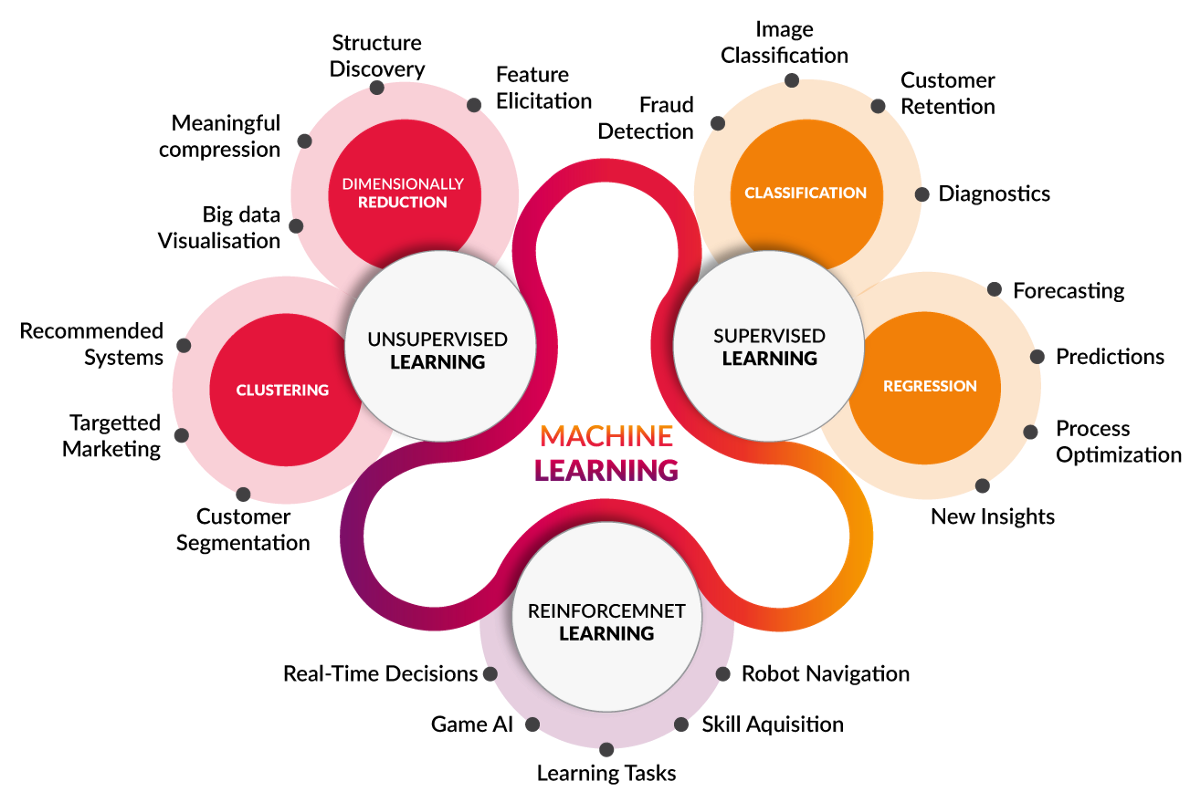
\includegraphics[width=\columnwidth]{images/MachineLearningTypes.png}
	\caption{Machine learning categories}
	\label{fig:mlcategories}
\end{figure}

We will now examine with a bird's eye view what the meaning of supervised and unsupervised learning is, and how they relate to the reinforcement learning methods.  

\subsection{Supervised Learning}

Supervised learning is probably the most widely used of the three main machine learning branches. The word \textit{supervised} comes from the fact that a supervisor, a teacher, is needed within the process. Supervised learning is obtained making an algorithm map input into output data, by first having a large set of training data: these are supervisors of the learning process, since for each given input set of date, the output set is already known. Therefore, the supervised learning is a non-linear function approximation. There are two main areas in which supervised learning is useful: \textit{classification problems} and \textit{regression problems}.
\\
\indent Classification problems are the ones in which the function has to map input data into an output class. For example, an usual classification task would be: given input images of a certain shape and size, tell which pictures contain cats or dogs. The function maps input data into a discrete set of outputs or categories, which come by definition as \textit{labeled} data.
\\
\indent Regression problems concern a more frequent machine learning problem, which is the mapping of input data into a real variable, which is a continuous output. For instance, we can think of a function approximation which, given the size in square meters, distance from the city center, number of rooms and age of a house in Shanghai, can predict its current value. In this case, a set of training data of real house values and their features has to be supplied to the learning algorithm, for predicting prices of houses that had not been seen before.


\subsection{Unsupervised Learning}
Unsupervised learning is learning when only input variables are given, and no outputs are available. The word \textit{unsupervised} comes from the fact that no supervisor is telling how good or bad the algorithm is performing. Therefore, the goal for these methods is to find the underlying structures and patterns in data. Unsupervised learning can be classified into two main subsets, \textit{association} and \textit{clustering}.
\\
\indent Association is about discovering common features in an unlabeled dataset: relationships between different entities can be found by measuring the frequencies of an occurrence in a dataset or with respect to other ones. Association uses probability distributions for measuring the correlation between objects: it is used for instance for giving recommendation on what to add to the checkout basket on a website, knowing behaviors of previous customers.
\\
\indent Clustering is a method for grouping data objects based only on information found in the data describing these objects and their relationship. Cluster analysis's goals are to maximize the similarity within objects in the same group and maximize the difference between objects in different groups: dissimilarities are measured in terms of a distance function and a weight is given to different features in order to provide a clear measure of how much the objects are alike. Clustering has many uses in real-world applications: i.e. the method can be used for identifying fake news, analyzing criminal activities or for personalization and targeting in marketing. 

\subsection{How is Reinforcement Learning different?}

Reinforcement Learning (RL) is a machine learning branch whose main purpose is to make machines learn from experience and make them decide actions to take. It differs from supervised learning since there is no direct need for labeled data: an RL agent could learn from direct interaction with the environment, by just observing the state it is in and a scalar reward (see next Section \ref{sec:elementsRL}). Besides, unlike unsupervised learning, its main purpose is not classification, rather taking decisions; for which unsupervised learning is not suitable.
\\
\indent An important remark about different machine learning methods has to be done though: even if Reinforcement Learning follows a different path with respect to the other machine learning branches, it is usually combined with them for obtaining either better performance or for achieving otherwise impossible results. That is why we will examine also Deep Neural Networks in Chapter \ref{ch:DNN}, which combined with Reinforcement Learning enhance it immensely and give birth to Deep RL, analyzed in Chapter \ref{ch:deeprl}.


\section{Elements of Reinforcement Learning} 
\label{sec:elementsRL}
The problem of reinforcement learning is at the core the interaction of an agent, that can be regarded as our robot, game AI, or even as a human being in a broader sense, which has to select actions on the environment in order to maximize a reward signal over time. In addition to the agent-environment interface which will be further discussed in Section~\ref{sec:MDP}, we can identify four main RL elements:
\begin{itemize}
	\item Policy
	\item Reward signal
	\item Value function
	\item Model
\end{itemize}
\indent The \textit{policy} defines how the agent behaves: in other words, it decides which actions should be selected given the circumstances. For instance, we can imagine Nintendo's arcade game \textit{Super Mario}, in which the hero has to complete levels by avoiding obstacles, beating enemies and jumping across holes in order to reach the flag ending the level or beating an enemy boss. In this scenario, we can consider the policy as the set of actions Mario will take for each situation, like running in a certain direction if there is an incoming foe or jumping with a desired trajectory when trying to overcome a crack in the ground.
\\
\indent The \textit{reward signal} is a scalar value the RL agent wants to maximize: for each time step, a reward signal will be given according to the current state. In the Super Mario example, a positive reward signal could be the score given to each desirable action, like beating an enemy or eating a power-up mushroom. If we want to make Mario avoid dangerous situations that could make him lose a life, we could give him a negative reward: therefore, the agent will try to avoid dangerous situations by trying to maximize the cumulative rewards. Thus, the reward signal is one of the most important tuning parts in a RL algorithm. Rewards can be tuned according to priorities. We could give a +1 reward for each time Mario gets a coin and a much more incisive -10 reward for each time he jumps into a hole; as a result we can make sure our hero will stay away from danger.
\\
\indent Whereas the reward defines what is good in a short time, the \textit{value function} defines what is good in the long run. It gives the value of how much reward the agent can accumulate in the future, starting from a particular state. Making the Mario game analogy, whereas rewards were the immediate scalar values for particular actions, the value of a state is much more farsighted: instead of focusing on a small and immediate reward for beating an insignificant enemy, Mario would rather focus more on a much higher reward in the future, like killing the boss of a level, thus giving up the small immediate reward.
\\
\indent Last but not least, the \textit{model} of an environment is a set of features of the environment itself, useful for easing the computations, predicting value functions and thus making the RL problem much easier to solve. Although models are very useful for planning, it is usual very difficult to craft them: in Super Mario, a model could be labels for each important object in the map and/or providing values of states in advance. Therefore, this one will be called a \textit{model-based} method, as opposed to the more used in RL \textit{model-free} methods, which do not require previous knowledge of the environment. This is because crafting the model itself, given a complicated game or a real-world scenario, could be actually more complex than developing the algorithm necessary for solving the RL problem.


\section{Thesis outline}

The purpose of this thesis is to demonstrate the ability of Reinforcement Learning in being able to control a system without information from any sensors, by just having access to raw visual input. This challenge will first require knowledge of the Reinforcement Learning theory described in Chapter \ref{ch:rl}, in particular about the Q-learning algorithm. In practice, iterative algorithms like Q-learning would need infinite computational power in a continuous state and/or action environment. Therefore, function approximators such as Deep Neural Networks(Chapter \ref{ch:DNN})have to be used for greatly reducing the computational requirements of the problem in mapping the state-action value functions. 
\\
\indent Combining together classical Reinforcement Learning and Deep Neural Networks gives birth to Deep Reinforcement Learning in Chapter \ref{ch:deeprl} which has proven suitable to a wide variety of tasks. After this initial dive into theory we will start in Chapter \ref{ch:CartPole} the real experimental challenge: the vision-based Cartpole balancing implementation in PyTorch using the OpenAI gym package for simulation. In Chapter \ref{ch:conclusion} possible future work that could take this thesis as a starting point will be explored.



